\subsection{CMA microbenchmark on Broadwell and TX2}
\label{sec:pa-microbenchmark}
In this subsection the CMA\_appinv microbenchmark is introduced and performance results from tests on the Intel Broadwell and Cavium ARM-based ThunderX2 architectures are presented.
In addition the performance of the microbenchmark when built with different compilers and runtime libraries is compared.

\subsubsection{CMA microbenchmark}

The GungHo dynamical model performs operations to solve
\begin{equation} \label{eq:matvec}
A \cdot \mathbf{x} = \mathbf{b}
\end{equation}
in various guises and contexts where $A$ is a matrix representing a partial differential equation, $\mathbf{b}$ is a vector containing information describing boundary conditions and $\mathbf{x}$ is a state vector.
The finite element methods that the GungHo application uses are written to perform operations on a cell-by-cell basis in what is termed Local Matrix Assembly (LMA).
The LMA microbenchmark discussed in Section \ref{sec:pa} is a characteristic example of such methods.
The LFRic infrastructure also contains methods for solving equation \ref{eq:matvec} on a column-by-column basis.
Although these Column Matrix Assembly (CMA) methods have yet to be utilised by the full GungHo application they are deployed in the gravity\_wave mini-app.

For this report a new CMA microbenchmark was generated using LFRic revision 15378 focused on the columnwise\_op\_appinv\_kernel\_code() routine in the gravity\_wave mini-app\footnote{At the time of writing the target kernel has not been significantly modified since extraction.}.
This kernel is used in the pre-conditioner for the Helmholtz solver to solve the tridiagonal case of equation \ref{eq:matvec} using the Thomas Algorithm~\cite{numericalrecipes}.
As per the LMA microbenchmark, the driver code was extracted from the Psyclone-generated Psy-layer and the kernel was taken directly from the LFRic source code.
By design, the driver routine contains the so called global optimisations, namely OpenMP worksharing and colouring (to prevent data race conditions) over columns on the sphere.

The dinodump capability from PYSKE was used to generate Known Good Output (KGO) which was use to verify the microbenchmark behaved as expected in later tests.
This involved adding additional PSYKE subroutine calls to the Psy-layer code in the gravity\_wave mini-app in order to capture the input scalars and arrays for the kernel.
The microbenchmark driver code was also trivially modified to read in the produced dinodump before calling the kernel and compare the result of the kernel against the KGO.
Before running the mini-app to generate the dinodump the number of vertical layers in the configuration was modified from the default (10) to 256.
While current NWP and climate GA and RA production configurations use between 70 and 90 vertical (UM) levels the microbenchmark was set to run over 256 layers in order to increase throughput and also in expectation that future configurations will run with increased vertical resolution.

While generating the new microbenchmark a minor bug in the kernel was discovered.
Specifically, the manner in which the kernel is called in gravity\_wave mini-app (and the supporting code comments) indicate that the kernel is called to update the target array but instead the kernel actually populates the array while overriding the initial contents.
It was confirmed by the original author of the code that the functionality of the kernel was correct and the comments are in error.
The bug has minimal performance impact on CPU architectures- an intent(inout) array should be intent(out)- but may have a larger impact on GPU architectures where the array would be being offloaded unnecessarily. 

The resultant microbenchmark can be found in the microbenchmark ~\cite{lfric-microbenchmarks} suite on GitHub.
Note that the LMA and CMA\_appinv microbenchmarks serve different purposes in the solver code and as such direct comparisons are not appropriate.

\subsubsection{CMA\_appinv performance}

Run times for the kernel on Intel Broadwell and Cavium ThunderX2 were measured using calls to \verb+omp_get_wtime()+.
In each case the kernel was run for 1000 iterations in order to obtain a smooth out runtime variability.
The latest stable version of each compiler on the two platforms were used.
Each executable was built with the \verb+-O3+ optimisation flag.

\begin{figure}
\centering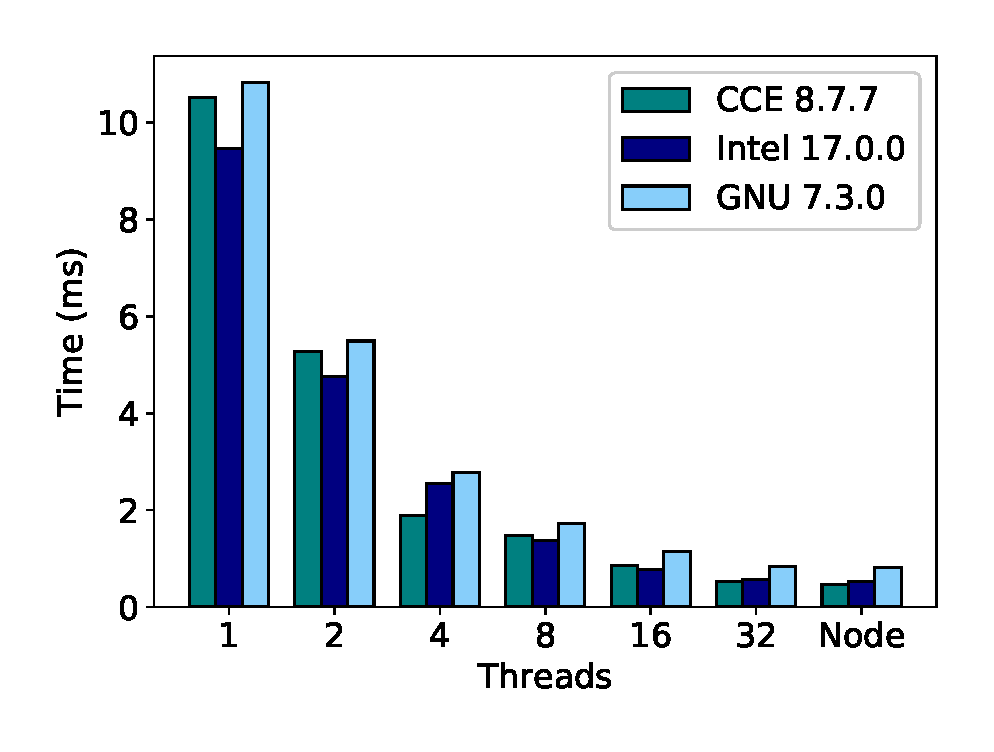
\includegraphics[scale=0.5]{figs/Broadwell_microbenchmark_vanilla.eps}
\caption{Thread-scaling of runtime on a Broadwell node. A lower time is better.}
\label{fig:cma_broadwell}
\end{figure}


\paragraph{Intel Broadwell} is the architecture in use for production NWP systems on the Met Office XC40 system.
Each node includes two 18-core 2.1 GHz processors.
On the XCS platform the compilers used were
\begin{itemize}
\item CCE 8.7.7
\item Intel 17.0.0.098
\item GNU 7.3.0
\end{itemize}

The runtimes of the CMA\_appinv microbenchmark when built with each of the three compilers on the Broadwell nodes are shown in figure \ref{fig:cma_broadwell}.

During the development of this work notable differences in performance between compiler versions became apparent.
For example, a measurable performance degradation between CCE 8.6.0 and the CCE 8.7.x series.
The single threaded (\$OMP\_NUM\_THREADS=1) runtime increased from 7.4s to 10.5s when changing between the two versions.
In other words CCE 8.6.0 produces a faster single-threaded executable than the Intel compiler but the 8.7.7 executable is slower than the Intel generated version.
This discrepancy is outwith the observed run-to-run variability on the system and is unexplained at present.

While the Intel compiled version outperforms CCE and GNU on a single thread, CCE gave the lowest runtime on a full node.
This could be a reflection of the better scalability of the Cray OpenMP runtime library c.f. Intel.

\paragraph{Cavium ThunderX2} processors, unlike some other ARM-based architectures, are targeted at the HPC market.
Each Isambard node includes two 32-core 2.1GHz processors: i.e. 64 cores per node vs the 36 cores of the Intel Broadwell nodes on XCS.
At the time of writing (after the March 2019 upgrade to CLE7.0) the supported compilers on the ARM-based nodes are
\begin{itemize}
\item CCE 8.7.9
\item Allinea 19.0.1
\item GNU 8.2.0
\end{itemize}
where the Allinea compiler is built on top of LLVM and Flang.
The runtimes of the CMA\_appinv microbenchmark when built with each of the three compilers on the ThunderX2 nodes are shown in figure \ref{fig:cma_tx2}.
Both single threaded and full node performance of the CCE built executable was found to be better than the Allinea and GNU built versions.

Note that the scale on the $y$ axis of figure \ref{fig:cma_tx2} is larger than that of figure \ref{fig:cma_broadwell} because the single-threaded performance of the benchmark on Broadwell is approximately 2 times better than on ThunderX2.
This marked difference disappears when performance on a full node (36/64 OpenMP threads) is considered.
In fact, in a node-for-node comparison the ThunderX2 out-performs Broadwell by approximately 15 per cent.


\begin{figure}
\centering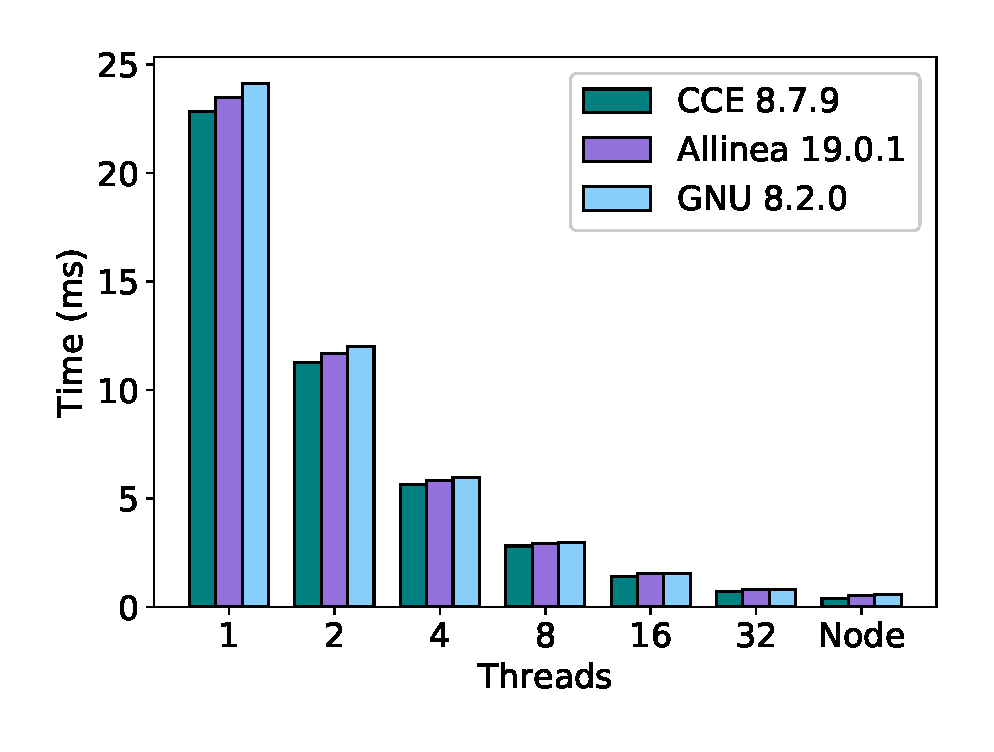
\includegraphics[scale=0.5]{figs/ThunderX2_microbenchmark_vanilla.eps}
\caption{Thread-scaling of runtime on a ThunderX2 node. A lower time is better.}
\label{fig:cma_tx2}
\end{figure}

\begin{table}[bh]
  \scriptsize
  \begin{center}
    \caption{Full node performance of the CMA\_appinv microbenchmark for the available compilers on the tested architectures.
      The best performing combination was CCE on ThunderX2.}
    \label{tab:cma_table}
     \begin{tabular}{|c|c|c|}
      \textbf{Compiler} & \textbf{Architecture} & \textbf{Runtime~(ms)} \\
      \hline
      CCE & Broadwell & 0.469 \\
      Intel & Broadwell & 0.517 \\
      GNU & Broadwell & 0.812 \\
      CCE & ThunderX2 & 0.398 \\
      Allinea & ThunderX2 & 0.558 \\
      GNU & ThunderX2 & 0.544 \\
    \end{tabular}
  \end{center}
\end{table}



\subsubsection{CMA\_appinv performance using drop-in library call}
Next it is investigated whether the implementation of the Thomas algorithm as written in the kernel can be replaced with a call to a standard library- in this case LAPACK.
The potential benefits of this include a potential improvement to runtimes of current architectures.
But, more importantly calling a standard API allows LFRic to tap into routines that have been optimised specifically for the architecture.
This could provide performance portability while reducing porting and maintenance costs when moving between future compute platforms.
A potential problem with this plan is that the memory layout used in the columnwise operator type objects differs from that expected by the tridiagonal solver in the LAPACK API.

A version of the microbenchmark using a call to the LAPACK \verb+dgtsv+ subroutine can be found in a branch named \verb+tridiagonal_lapack+.
Further investigation showed that runtime performance (single threaded and full node) was poor compared to the baseline microbenchmark.
While the thread-scaling of the original application was maintained, the runtime increased by approximately 50-80 per cent (depending on the compiler used).
A significant fraction of this slow-down was due to the aforementioned memory copies from the ``LFRic-shaped'' arrays into the ``LAPACK-shaped'' arrays and back.
To demonstrate this the new version of microbenchmark was produced in which the costly memory copies had been removed.
While this obviously produces scientifically nonsensical results, this version can be used to quantify the costs of the memory copies.

The runtimes for the three variants of microbenchmark (the baseline version, the LAPACK version and the LAPACK version without any memory copies) are shown in figure \ref{tab:lapack_table}.
From this one can infer that the increase in runtime is not solely due to the memory copies.
Instead, even when the memory transfer costs have been negated the LAPACK version of the kernel does not perform as well as the trunk version on either Broadwell or ThunderX2.
Investigations confirmed that this result held regardless of whether the Cray-libsci package or the Intel MKL package was linked against.
It is believed that the lack of performance of the LAPACK version is in part due to the fact that these implementations have been optimised for larger matrix problems (than 256x256).
At this time replacing the implementation of the Thomas algorithm with the LAPACK version would not beneficial to LFRic performance on Broadwell or ThunderX2 architectures.

\begin{table}[t]
  \scriptsize
  \begin{center}
    \caption{Single threaded runtimes for the three variants of microbenchmark when built with different compilers.}
    \label{tab:lapack_table}
     \begin{tabular}{|c|c|c|c|c|c|}
      \textbf{Compiler} & \textbf{Architecture} & \textbf{Base~(ms)} & \textbf{LAPACK~(ms)} & \textbf{LAPACK no copies~(ms)} \\
      \hline
      CCE & Broadwell & 10.517 & 15.382 & 12.003 \\
      Intel & Broadwell & 9.475 & 15.765 & 12.309 \\
      GNU & Broadwell & 10.832 & 18.271 & 14.242 \\
      CCE & ThunderX2 & 22.835 & 36.839 & 33.691 \\
      Allinea & ThunderX2 & 23.464 & 38.452 & 34.876 \\
      GNU & ThunderX2 & 24.133 & 34.317 & 29.921 \\
    \end{tabular}
  \end{center}
\end{table}
